\begin{figure}[H]
    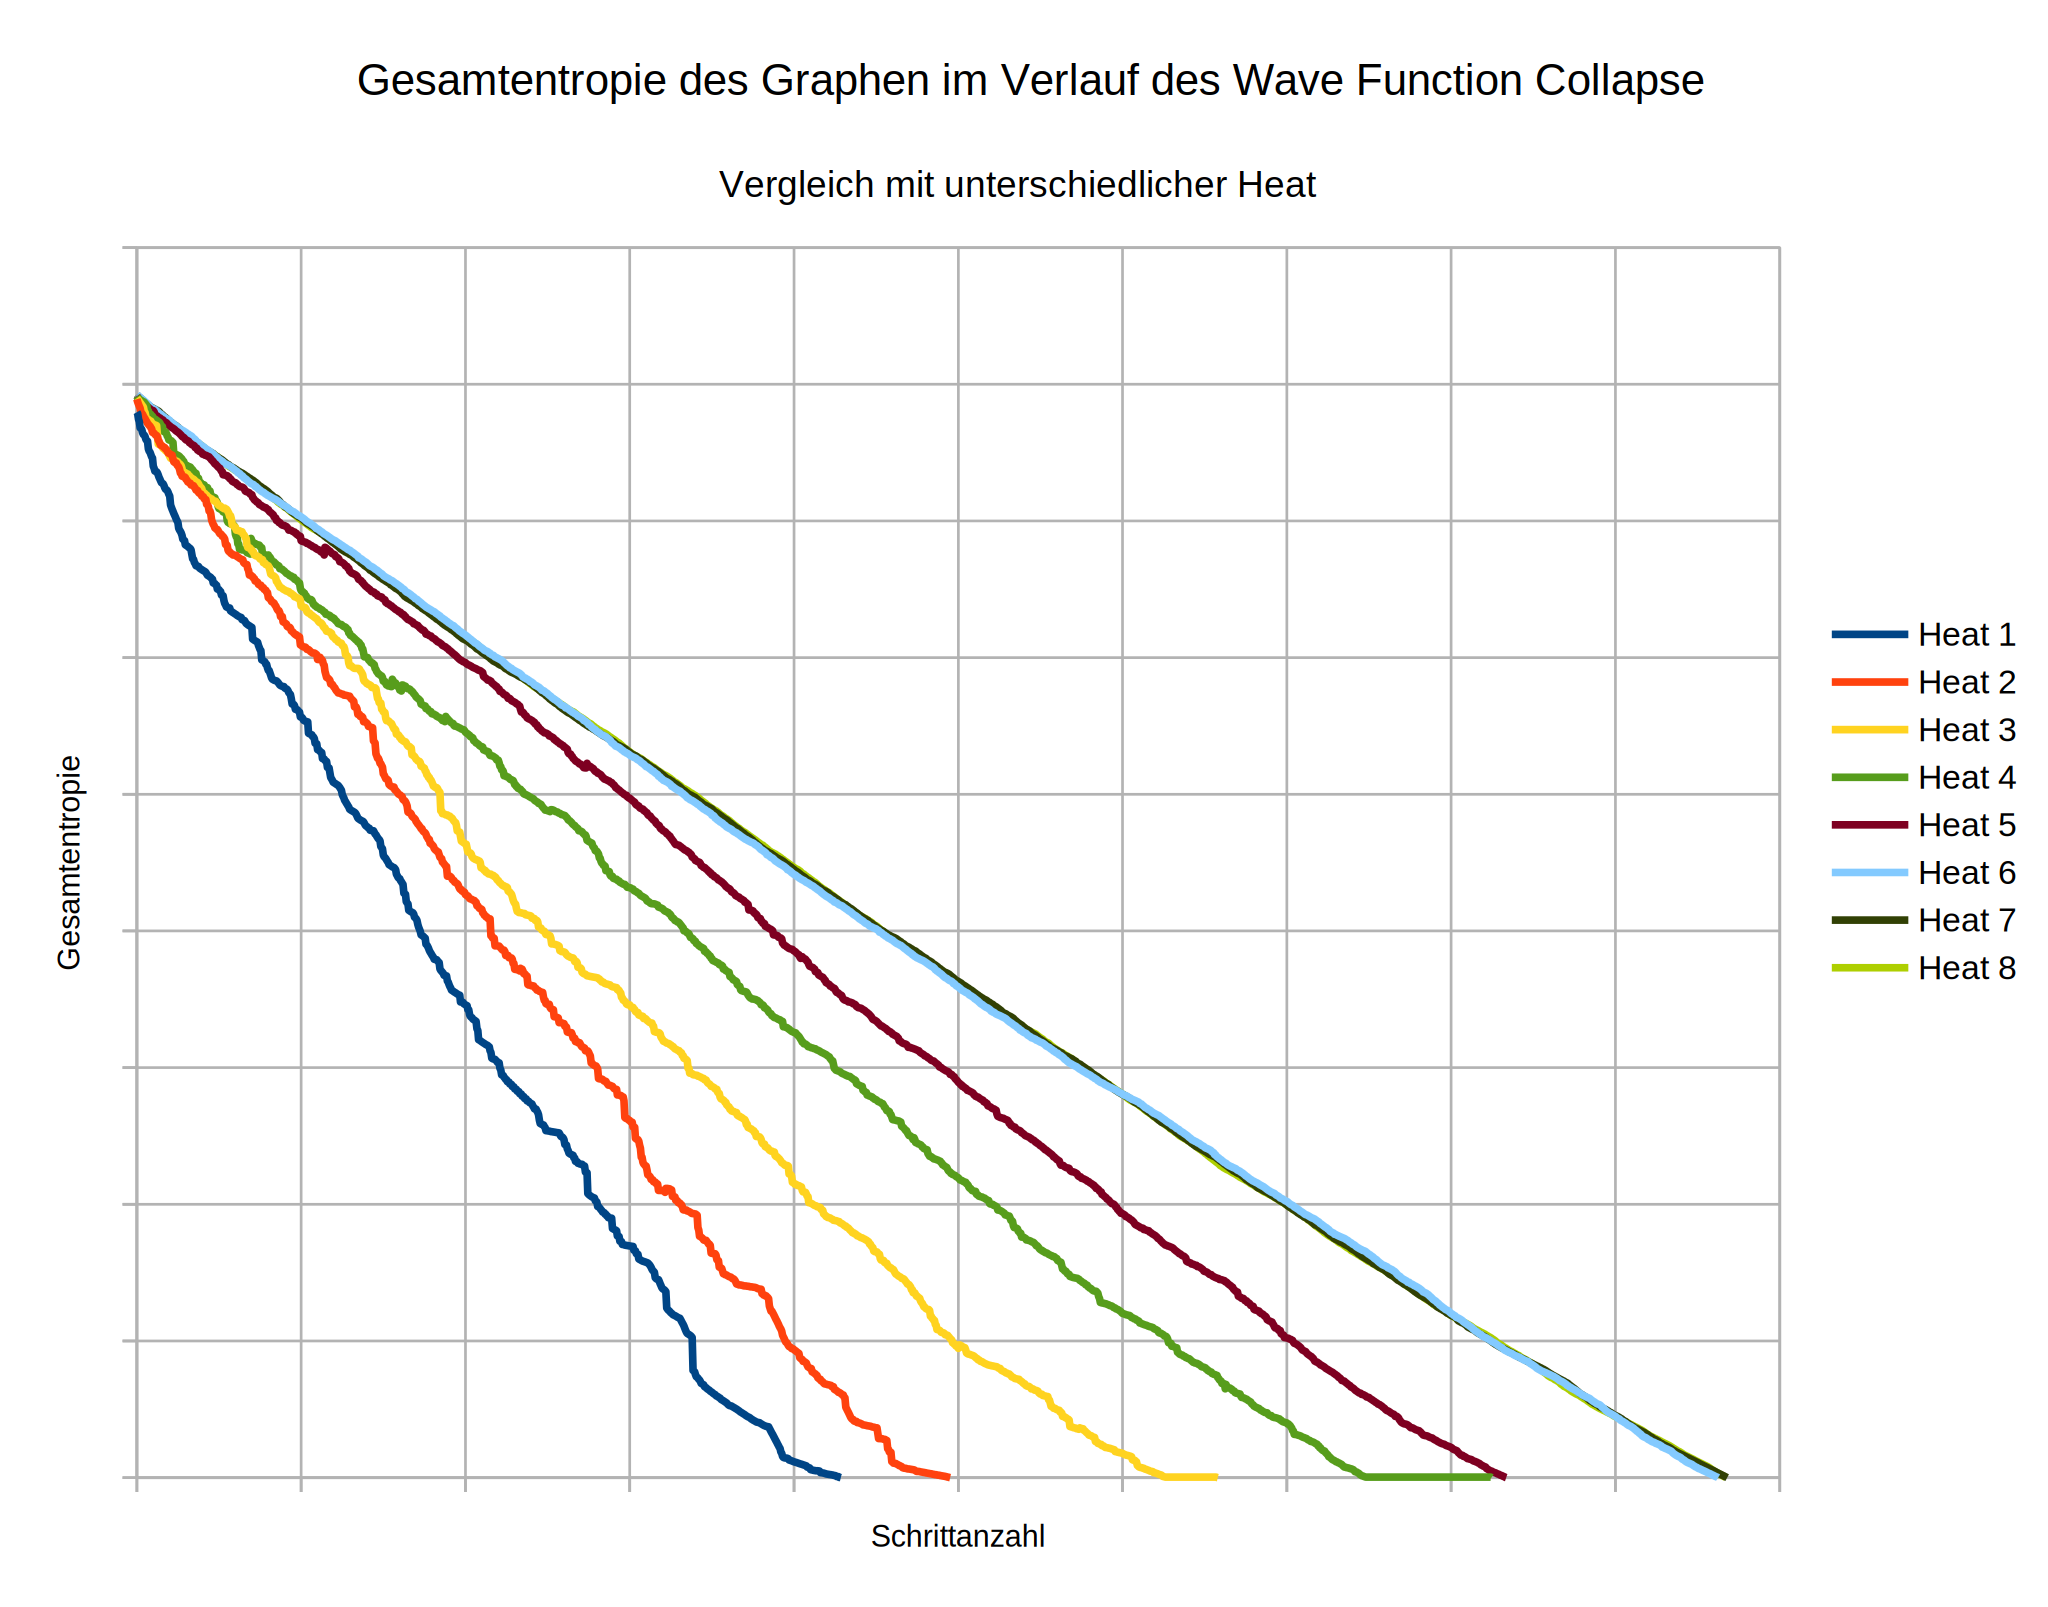
\includegraphics[width=\linewidth]{data/ms_algorithm/1.png}
    
    \caption{
         Ablauf des Model Synthesis Algorithmus \cite{merrel}.
         Das Modell wird mit leeren Bauteilen initialisiert. Dann werden Ausschnitte(rot) geleert und jedem Knotenpunkt werden alle Bauteile zugewiesen. Jedem Knotenpunkt wird ein Bauteil zugewiesen, so dass der Ausschnitt konsistent bleibt. Der nächste Ausschnitte überschneidet sich mit der ersten. Der Algorithmus ist fertig wenn alle Knotenpunkte verändert wurden.
    }
    \label{fig:ms_algorithm}
\end{figure}